\documentclass[12pt,a4paper]{article}
\usepackage[utf8]{inputenc}
\usepackage[spanish]{babel}
\usepackage{amsmath}
\usepackage{amsfonts}
\usepackage{amssymb}
\usepackage{graphicx}
\usepackage[left=2cm,right=2cm,top=2cm,bottom=2cm]{geometry}
\author{Enciso Guerrero Benjamin Salvador\\
Carlos Enrrique Moran Garabito\\
Cinematica De Robots }
\title{Angulos de Euler}
\begin{document}
\maketitle

\includegraphics[scale=1.8]   {upzmgg.jpg}
\newpage
Angulos de Euler\\\\
Los ángulos de Euler (j,q,y) están definidos para todas las configuraciones, excepto para el caso en que los ejes z1,z sean paralelos. Si este estado se mantiene durante intervalos extensos de tiempo, el sólido experimenta realmente un movimiento con un eje fijo, y sólo se necesita un parámetro para posicionarlo. Si el paralelismo es un hecho puntual, pueden definirse los ángulos de Euler por continuidad temporal.\\\\Se va a proceder a continuación a construir la posición de la base móvil a partir de la fija y los tres ángulos de Euler, suponiendo que no se dan las condiciones de degeneración aludidas en el párrafo anterior. Este proceso se realizará mediante tres rotaciones sucesivas que irán transformando la terna {i1,j1,k1} en la {n,u1,k1}, {n,u,k} y la {i,j,k}.\\\\\\\
Rotaciones de Euler\\\\
Una vez determinada la posición del sólido con punto fijo mediante los ángulos de Euler, se va a expresar su rotación en función de estos ángulos.\\
La base {n ,k1, k} se denomina base de Euler y las componentes de la rotación del sólido en dicha base, reciben el nombre de rotaciones de Euler, resultando que son las derivadas de los ángulos de Euler respecto al tiempo.
Las rotaciones de Euler  reciben los nombres de nutación, precesión y rotación propia .\\
En algunas ocasiones es necesario utilizar las componentes de rotación en la base móvil\\\\
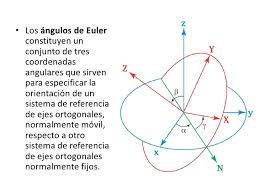
\includegraphics[scale=1.8]{li.jpg} \\
\newpage 
Posición de un sólido con un punto fijo: ángulos de Euler\\\\
Cuando un sólido experimenta un movimiento plano, sólo se necesitan tres parámetros para determinar su posición. Cuando el sólido gira en torno a un eje fijo, sólo es necesario un`parámetro para determinarla. Cuando se conoce la posición de un punto fijo del sólido, entonces sólo se necesitan tres parámetros para determinar su posición.\\\\
Es inmediato reducir el problema de la determinación de la posición de un sólido con un punto fijo al de la determinación de la posición de una referencia tridimensional vinculada al sólido, pues conocida ésta, los puntos del sólido se ubican mediante sus coordenadas que son constantes. Se trata de determinar los tres vectores de una base ortonormal considerada móvil respecto a una referencia fija.\\\\
En principio se tienen nueve parámetros (las componentes de los tres vectores móviles en la base fija), pero las condiciones debidas a la ortonormalidad de la base imponen seis restricciones más, a saber, que los tres vectores han de ser unitarios y que deben ser perpendiculares entre sí. Quedan, pues, tres únicos parámetros para determinar la posición de la base móvil respecto a la fija. Estos tres parámetros pueden elegirse de entre una gran variedad de ellos, pero los más frecuentes son los ángulos de Euler, que se procede a definir.
\\\\
Matrices de rotación y velocidad angular
\\\\
A partir de la relación entre los ángulos de Euler y el movimiento de los soportes de Cardano, se puede probar que todo sistema de coordenadas puede ser descrito con los tres ángulos de Euler. Si llamamos ( R ) a la matriz de rotación tridimensional que representa la transformación de coordenadas desde el sistema fijo al sistema móvil, el teorema de Euler sobre rotaciones tridimensionales, afirma que existe una descomposición única en términos de los tres ángulos de Euler.
\\\\
Ángulos de Tait-Bryan
\\\\
Muchas veces en ingeniería aeronáutica se utiliza el nombre de ángulos de Euler para hablar de los ángulos que en geometría se conocen como ángulos de Tait-Bryan (por el matemático escocés Peter Guthrie Tait (1831-1901)).
\\\\Estos ángulos se prefieren en aeronáutica porque le asignan un ángulo de inclinación cero a un avión en horizontal, a diferencia de los ángulos de Euler que le asignarían 1/2. Estos ángulos también definen una rotación de forma única alrededor de cada uno de los ejes intrínsecos del objeto. Sin embargo, como ambas son formas de expresar la orientación de un cuerpo, existe una relación entre ellos; pudiéndose expresar unos en función de otros mediante una matriz de transformación.

\end{document}